\section{Background and Motivation}


% Outline
% Review the profiling methods/concepts in prior work.
% Peripheral papers
%   1. How they manage to do peripheral operations?
%   2. Are they supposed to fail in our scenarios?


\subsection{Intermittent Peripheral Operations}

% Intro
% While prior work in intermittent computing have been able to efficiently maintain forward progress on computational workloads, intermittent peripheral operations are not widely studied. 
% This is typically achieved by carefully saving volatile computing state (e.g. data in CPU registers, SRAM) into NVM before a power failure, and restoring it on power recovery. 
% Some of the published approaches intrinsically guarantee the atomicity and termination of peripheral operations, while others focus on computational workloads without support for peripherals. 
Several papers have been published on handling atomic peripheral operations in intermittent systems, where energy profiling of workloads is an inherent part of their methodologies.

% Review of papers about or support peripherals
%   Karma? Sytare?

% DEBS
DEBS~\cite{gomez2016dynamic} experimentally profiles the energy consumption of each task at design time, and designates a threshold to each task individually.
DEBS enters a low-power mode (LPM) after completing an operation, and waits for energy replenishment until the next threshold. 

% Samoyed, Alpaca?
Samoyed~\cite{maeng2019supporting} utilizes a custom design-time \textit{energy profiler}~\cite{colin2016energy-interference-free} to identify whether the adopted energy storage size suffices to run an adequate number (hundreds, as suggested) of peripheral operations in one energy cycle. 
At runtime, Samoyed starts execution when energy is refilled to a certain threshold, and keeps executing until energy is depleted. 
% Samoyed is a proactive approach where the program knows the boundaries of atomic operations, such that it only outputs valid data on the completion of an atomic operation and disables checkpoints during execution. 
Samoyed differs from most static approaches, e.g. Alpaca, on handling computational workloads where it reactively checkpoints when energy falls below a low threshold, and supports user-customized subdivision of peripheral operations when the operation cannot complete in one energy cycle. 

% RESTOP (similar to re-execution)
RESTOP~\cite{rodriguez2018restop} provides programmer-configurable rules that track the instructions issued to peripherals through serial interfaces in a history table.
On power recovery, RESTOP re-issues instructions saved in the history table and then resumes the interrupted operation. 
At design time, RESTOP needs to profile the worst-case energy consumption for restoring peripheral state to identify the minimum (most-efficient) restore threshold. 

% Adaptive?
% Online profiling but inefficient



Prior work profiles the energy consumption of each atomic operation at design time to determine a voltage threshold or a capacitor size that ensures forward progress. 
However, this does not guarantee the completion of every atomic operation because energy consumption can change with any runtime conditions different to the profiling setup (detailed in Section~\ref{subsec:dynamic_energy_consumption}). 
Hence, previous designs typically achieve atomicity by carefully managing the system state, such that the atomic operation does not output valid data until completion, and, if a power failure happens during the operation, the system state rolls back to the start of the operation upon power recovery (rather than checkpoint and resume). 
Also, previous designs should usually leave an inefficiently safe margin between the profiled energy consumption and the energy to be allocated, such that dynamic variation can be largely tolerated. 



% Comments: 
% All previous work involves a design-time energy profiling of workloads.




% Comments: Justify Samoyed, DEBS for comparisons in this paper? 

\subsection{Variability in Energy Consumption, Storage, and Input} \label{subsec:dynamic_energy_consumption}


We took an example of atomic operations to study the dynamic variation of energy consumption. We chose the AES accelerator on TI MSP430FR5994, running a data encryption peripheral function. 

Explain each kind of dynamic variation of energy consumption, as listed in Section I-A.

\subsubsection{Capacitor Degradation and Tolerance}

\subsubsection{Data size}


\begin{figure}[!t]
    \centering
    \begin{tikzpicture}
    \begin{axis}[
            width=1.0\columnwidth,
            height=5cm,
            ymin=0,
            ymax=200,
            xmin=0,
            xmax=4,
            xlabel=Data Size (KiB),
            ylabel=$\Delta V_{\text{task}}$ (mV),
            legend style={at={(0.05,0.95)},
            anchor=north west,legend columns=1},
        ]
        \addplot
            plot [black,only marks]
            table [x=data_size, y=voltage_drop,col sep=comma] {ch5_repta/figures/variable_data/variable_data.csv};
        \addplot
            plot [black]
            {44.3 * x + 16.9};
        \legend{Measurements, Linear Fit}
    \end{axis}
    \end{tikzpicture}
    \caption{Voltage drop vs data size.}
    \label{fig:variable_datasize}
\end{figure}

Figure~\ref{fig:variable_datasize}

\subsubsection{Peripheral Configurations}

Table~\ref{tab:configurations}

\begin{table}[!t]
    \renewcommand{\arraystretch}{1.2}
    \centering
    \caption{Peripheral configuration variability, AES Encryption 4KB}
    \label{tab:configurations}
    \begin{tabular}{|c|c|}
    \hline
    \textbf{Configuration} & \textbf{$\Delta V_{\text{task}}$}\\
    \hline
    128-bit key & \SI{194}{\milli\volt}\\
    192-bit key & \SI{230}{\milli\volt}\\
    256-bit key & \SI{245}{\milli\volt}\\
    \hline
    \end{tabular}
\end{table}

\subsubsection{Device}

Table~\ref{tab:device}

\begin{table}[!t]
    \renewcommand{\arraystretch}{1.2}
    \centering
    \caption{Device variability, AES 128-bit Encryption 4KB}
    \label{tab:device}
    \begin{tabular}{|c|c|c|c|}
    \hline
    \textbf{Device No.} & \textbf{$\Delta V_{\text{task}}$} & \textbf{System Capacitance} & \textbf{Time} \\
    \hline
    % 1 & \SI{764}{\micro\ampere}\\
    % 2 & \SI{773}{\micro\ampere}\\
    % 3 & \SI{756}{\micro\ampere}\\
    1 & \SI{185}{\milli\volt} & \SI{29}{\micro\farad} & \SI{6.444}{\milli\second} \\
    2 & \SI{194}{\milli\volt} & \SI{35}{\micro\farad} & \SI{6.479}{\milli\second} \\
    3 & \SI{179}{\milli\volt} & \SI{29}{\micro\farad} & \SI{6.462}{\milli\second} \\
    \hline
    \end{tabular}
\end{table}

\subsubsection{Other}
Clock frequency (Tentative). 1MHz: 757uA (This should be checked later as it takes the same time to complete).

% \subsection{To operate at a lower voltage}

\subsubsection{Voltage}

(This should be relevant as you mention it's better to operate at lower voltage)


% Prior experiment

% 2.1V: 750uA

% 2.4V: 755uA

% 2.7V: 763uA

% 3.0V: 763uA

% 3.3V: 764uA

% 3.6V: 764uA


% New experiment

| Start V | End V | Delta V |

| 2.020V        | 1.836V      | 184mV   |

| 2.102V        | 1.917V      | 185mV   |

| 2.214V        | 2.030V      | 184mV   |

| 2.301V        | 2.117V      | 184mV   |

| 2.424V        | 2.240V      | 184mV   |

| 2.542V        | 2.352V      | 190mV   |

| 2.634V        | 2.444V      | 190mV   |

| 2.710V        | 2.521V      | 189mV   |

| 3.360V        | 3.166V      | 194mV   |

% Figure~\ref{fig:voltage}
% \begin{figure}[!h]
%     \centering
%     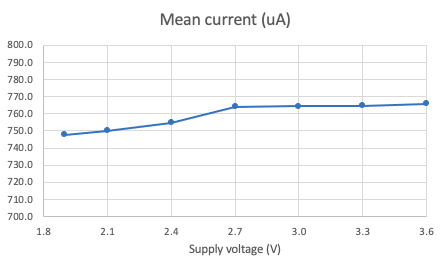
\includegraphics[width=3.49in]{voltage.jpg}
%     \caption{Current consumption vs voltage. }
%     \label{fig:voltage}
% \end{figure}

\subsubsection{Charging efficiency of energy harveser vs Vcc}

\begin{figure}[!t]
    \centering
    \begin{tikzpicture}
    \begin{axis}[
            width=1.0\columnwidth,
            height=5cm,
            ymin=0,
            ymax=130,
            xmin=0,
            xmax=5.3,
            xlabel=Voltage (V),
            ylabel=Current (\SI{}{\micro\ampere}),
            legend style={at={(0.05,0.05)},
            anchor=south west,legend columns=1},
        ]
        \addplot
            plot [black,only marks]
            table [x=v, y=i,col sep=comma] {ch5_repta/figures/pv_curve/pv_curve.csv};
        \addplot
            plot [black,ultra thick]
            {-7.2 * x + 124.4};
        \legend{Measurements, Linear Fit for \SIrange{0}{4}{\volt}}
        % \legend{Measurements}
    \end{axis}
    \end{tikzpicture}
    \caption{IV curve.}
    \label{fig:pv_iv}
\end{figure}


% \subsection{Infeasibility Offline Profiling}

% As shown in Section~\ref{subsec:dynamic_energy_consumption}, dynamic current consumption is in existence across the variation of devices, clock frequencies, supply voltage, and temperature.





% Simulation
\subsection{Forward Progress Improvement with Adaptive Energy Budgeting}

We took a modelling process to demonstrate the potential of improving forward progress with adaptive energy budgeting, given dynamic execution time and dynamic current draw.

\subsubsection{Model Description}
We modelled an ideal case of adaptive energy budgeting, where the system exactly knows how much time the next atomic operation will take and how much the current draw is. The system sets a voltage threshold that exactly guarantees the charge consumption even if the supply current immediately drops to zero after the start of an operation. 

\subsubsection{Simulation Setup}
The system has a \SI{10}{\micro\farad} capacitor for buffering energy with \SI{1.5}{\volt} charge at the beginning. 
The system consumes \SI{20}{\micro\ampere} in the LPM and \SI{0}{\micro\ampere} when off.
The shutdown threshold is \SI{1.8}{\volt}, which is also the end voltage that all approaches are profiled for or adapted to. 
We set a dummy workload which draws \SI{750}{\micro\ampere} and takes up to \SI{5}{\milli\second} to complete.
Two sets of simulation were conducted.
One set was run with a randomized dynamic execution time that is uniformly distributed between 0 and \SI{5}{\milli\second}, with \SI{750}{\micro\ampere} current draw unchanged. The other was run with a dynamic current draw which is increased by 0-20\% uniformly distributed, with \SI{5}{\milli\second} execution time. 
We ran each set of simulation for 10 times and took the mean, maximum, and minimum of the number of completed operations as a metric of forward progress. 

\subsubsection{Results}

Figure~\ref{fig:model_time}.

\begin{figure}[t]
    \centering
    \begin{tikzpicture}
    \begin{axis}[
        width=1.0\columnwidth, height=5cm,
        ybar,
        ymin=0,
        ymax=600,
        enlarge x limits=0.3,
        legend style={at={(0.5,1.2)},
        anchor=north,legend columns=-1},
        ylabel={No. completions},
        symbolic x coords={\SI{100}{\micro\ampere},\SI{300}{\micro\ampere},\SI{500}{\micro\ampere}},
        xtick=data,
    ]
    % Samoyed
    \addplot
        plot [black,fill=Set1-A,postaction={pattern=dots},error bars/.cd,y dir=both,y explicit]
        table [x=current,y=samoyed_perf,y error plus=samoyed_perf_err+, y error minus=samoyed_perf_err-, col sep=comma] {ch5_repta/figures/model_time/model_time.csv};
    % DEBS
    \addplot
        plot [black,fill=Set1-B,postaction={pattern=north east lines},error bars/.cd,y dir=both,y explicit]
        table [x=current,y=debs_perf,y error plus=debs_perf_err+, y error minus=debs_perf_err-, col sep=comma] {ch5_repta/figures/model_time/model_time.csv};
    % Adaptive
    \addplot
        plot [black,fill=Set1-C,postaction={pattern=north west lines},error bars/.cd,y dir=both,y explicit]
        table [x=current,y=opta_perf,y error plus=opta_perf_err+, y error minus=opta_perf_err-, col sep=comma] {ch5_repta/figures/model_time/model_time.csv};
    \legend{Samoyed, DEBS, Adaptive}
    \end{axis}
    \end{tikzpicture}
    \caption{Dynamic execution time.}
    \label{fig:model_time}
\end{figure} 


Figure~\ref{fig:model_current}.
\begin{figure}[t]
    \centering
    \begin{tikzpicture}
    \begin{axis}[
        width=1.0\columnwidth, height=5cm,
        ybar,
        ymin=0,
        ymax=250,
        enlarge x limits=0.3,
        legend style={at={(0.5,1.2)},
            anchor=north,legend columns=-1},
        ylabel={No. completions},
        symbolic x coords={\SI{100}{\micro\ampere},\SI{300}{\micro\ampere},\SI{500}{\micro\ampere}},
        xtick=data,
        ]
        % Samoyed
        \addplot
            plot [black,fill=Set1-A,postaction={pattern=dots},error bars/.cd,y dir=both,y explicit]
            table [x=current,y=samoyed_perf,y error plus=samoyed_perf_err+, y error minus=samoyed_perf_err-, col sep=comma] {ch5_repta/figures/model_current/model_current.csv};
        % DEBS
        \addplot
            plot [black,fill=Set1-B,postaction={pattern=north east lines},error bars/.cd,y dir=both,y explicit]
            table [x=current,y=debs_perf,y error plus=debs_perf_err+, y error minus=debs_perf_err-, col sep=comma] {ch5_repta/figures/model_current/model_current.csv};
        % Adaptive
        \addplot
            plot [black,fill=Set1-C,postaction={pattern=north west lines},error bars/.cd,y dir=both,y explicit]
            table [x=current,y=opta_perf,y error plus=opta_perf_err+, y error minus=opta_perf_err-, col sep=comma] {ch5_repta/figures/model_current/model_current.csv};
        \legend{Samoyed, DEBS, Adaptive}
    \end{axis}
    \end{tikzpicture}
    \caption{Dynamic current draw.}
    \label{fig:model_current}
\end{figure} 
    

Analyse where the improvement comes from (probably with a voltage trace).